%! LuaLaTeX 文書
\documentclass[unicode,colorlinks]{beamer}
\usetheme{metropolis}
\usefonttheme{professionalfonts}

\hypersetup{linkcolor=blue,urlcolor=teal}

\usepackage{luatexja}
\ltjsetparameter{jacharrange={-2,-3,-8}}
\usepackage[no-math,match,deluxe]{luatexja-preset}

\usepackage{graphicx,xcolor}
\usepackage{pxrubrica}
\usepackage{tcolorbox}
\usepackage{bxwareki}

\usepackage{tikz}
\usetikzlibrary{plotmarks}

\usepackage{bxokumacro}
\usepackage{keystroke}

\usepackage[T1]{fontenc}
\usepackage{amsmath,mathtools,amssymb,mathrsfs,rsfso,mleftright}
\usepackage[math]{kurier}
\usepackage[euler-digits]{eulervm}
\usepackage[scaled]{beramono}
\allowdisplaybreaks[4]

%%%%%%%%%% 商用フォントを用いているので、自分でタイプセットする場合は適当に以下を変えてください
\setmainfont[
	Ligatures=TeX,
	BoldFont=FOT-RodinNTLGPro-EB,
	ItalicFont=FOT-RodinNTLGPro-EB,
]{FOT-RodinNTLGPro-B}
\setsansfont[
	Ligatures=TeX,
	BoldFont=FOT-RodinNTLGPro-EB,
	ItalicFont=FOT-RodinNTLGPro-EB,
]{FOT-RodinNTLGPro-B}
\setmainjfont[
	Ligatures=TeX,
	CharacterWidth=Proportional,
	JFM=prop,
	BoldFont=FOT-RodinNTLGPro-EB,
	ItalicFont=FOT-RodinNTLGPro-EB,
]{FOT-RodinNTLGPro-B}
\setsansjfont[
	Ligatures=TeX,
	CharacterWidth=Proportional,
	JFM=prop,
	BoldFont=FOT-RodinNTLGPro-EB,
	ItalicFont=FOT-RodinNTLGPro-EB,
]{FOT-RodinNTLGPro-B}
\setmonofont[
	Ligatures=TeX
]{DejaVu Sans Mono}
\setmonojfont[
	Ligatures=TeX,
]{NotoSansMonoCJKjp-Regular}

%%%%%%%%%% 以下は自前コマンド

\newcommand{\centeralign}[1]{\rule{0pt}{0pt}\hfill#1\hfill\rule{0pt}{0pt}}
\newcommand{\Unit}[1]{\,\mathrm{#1}}

\setlength{\parskip}{2ex}

\title{大気放射の基礎\\--Liou著 藤枝・深堀訳 (2014) の講読--}
\author{北海道大学理学部 人見祥磨}
\date{\warekitoday}

\begin{document}
\maketitle
\mleftright

\begin{frame}{目次}
	\tableofcontents
\end{frame}

\section{動機}

\begin{frame}{動機}
	\begin{itemize}
		\item 惑星大気の熱輸送について興味があった
		\item 惑星大気について、自転周期や地軸の傾きによって、
			どのように熱輸送が変化するかシミュレーションしたい
		\item そのために、大気の温度分布を知りたい
		\item 放射に関する基本的な事項の知識の確認
		\item 放射に関して、観測なども含めて、基礎事項を解説している Liou の教科書を
			読むことにした
			\begin{itemize}
				\item 大気放射学 {\scriptsize---衛星リモートセンシングと気候問題へのアプローチ---}\\
					K.N.Liou(著) 藤枝 鋼、深堀 正志(翻訳)\\
					共立出版 \textbf{(2014)} 672ページ
			\end{itemize}
	\end{itemize}
\end{frame}

\section{放射伝達方程式の基礎}

\begin{frame}{放射伝達方程式}
	放射伝達強度 $I_\lambda^\mathrm{d}$ が、放射の伝搬方向に厚さ $ds$ で密度 $\rho$ の媒質を横切った後に、
	$I_\lambda^\mathrm{d}+dI_\lambda^\mathrm{d}$ になるとする
	\[dI_\lambda^\mathrm{d}=-k_\lambda\rho i_\lambda\,ds\]
	$k_\lambda$ は質量消散断面積と呼ばれる

	射出と多重散乱による放射強度の増加が以下で与えられるように、
	放射源係数 $j_\lambda$ を定義する
	\[dI_\lambda^\mathrm{s}=j_\lambda\rho\,ds\]
\end{frame}

\begin{frame}{放射伝達方程式}
	ふたつの式を関連付けて、
	\[dI_\lambda=dI_\lambda^\mathrm{d}+dI_\lambda^\mathrm{s}=-k_\lambda\rho I_\lambda\,ds+j_\lambda\rho\,ds\]

	放射源関数 $J_\lambda\equiv j_\lambda/k_\lambda$ を導入すると、
	\[\frac{dI_\lambda}{k_\lambda\rho\,ds}=-I_\lambda+J_\lambda\quad\text{……放射伝達方程式}\]
\end{frame}

\begin{frame}
	\section{スペクトル線の広がり}
	単色の放射は、相互作用により非単色となり、有限の幅を持つスペクトル線となる
\end{frame}

\begin{frame}
	\frametitle{スペクトル線の広がり}
	単色の射出は現実には観測されない

	原子や分子への外部からの影響と、射出の際のエネルギー損失のため、
	エネルギー遷移する間にエネルギー準位が僅かに変化する

	その結果、非単色の放射となり、有限の幅を持つスペクトル線が観測される
\end{frame}

\begin{frame}
	\frametitle{ローレンツ線形}
	\begin{description}
		\item[ローレンツ線形] 衝突によって広げられたスペクトル線の線形
	\end{description}

	\begin{columns}
		\begin{column}{0.6\textwidth}
			\[k_\nu=\frac{S}{\pi}\frac{\alpha}{(\nu-\nu_0)^2+\alpha^2}=Sf[\nu-\nu_0]\]
		\end{column}
		\begin{column}{0.3\textwidth}
			\centeralign{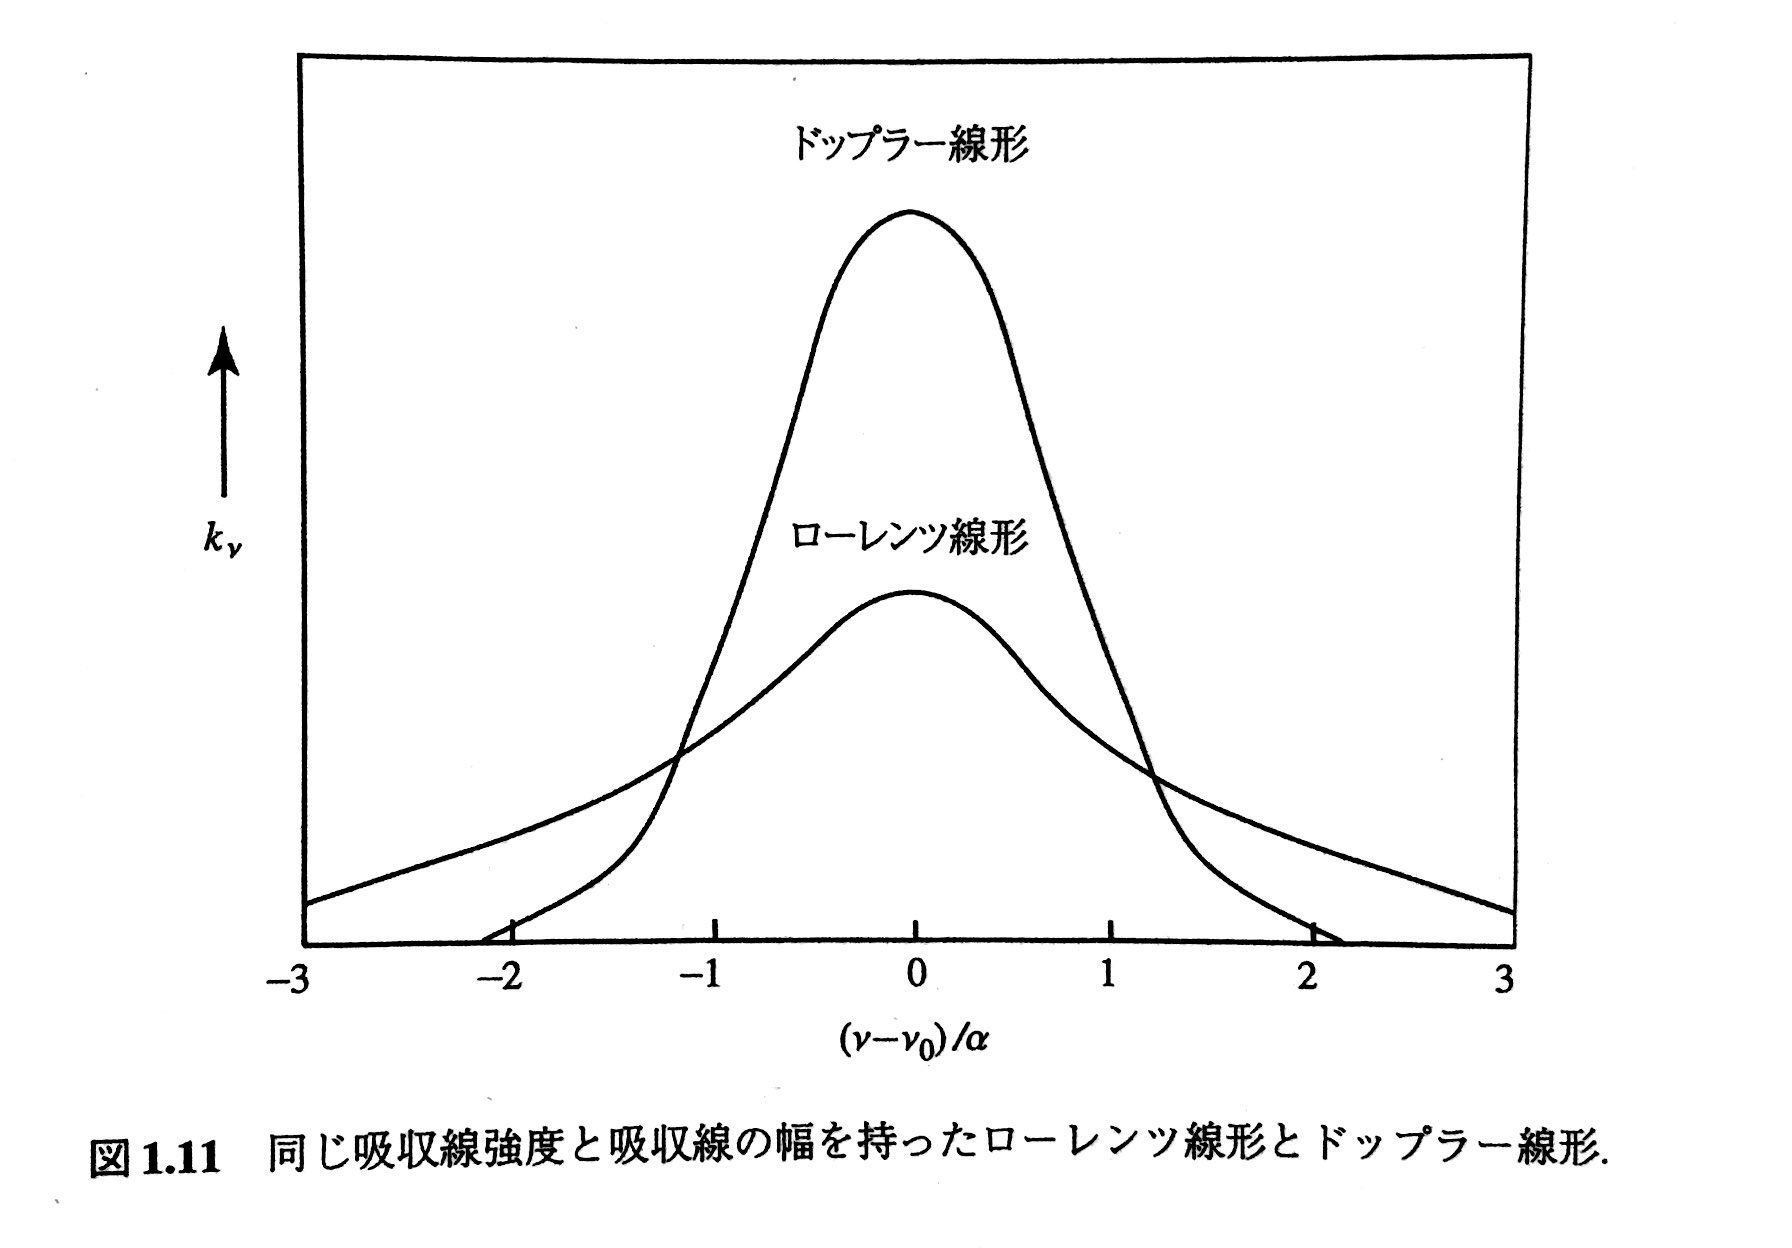
\includegraphics[width=\textwidth]{lorentz.jpg}}
		\end{column}
	\end{columns}

	$k_\nu$: 吸収係数 ;\quad
	$\nu_0$: 理想的な単色の吸収線の波数;\\
	$\alpha$: 吸収線の半値半幅(圧力と温度の関数);\\
	$f$: 形状因子 (shape factor);\quad
	$\displaystyle S=\int^\infty_{-\infty}k_\nu\,d\nu$: 線強度
\end{frame}

\begin{frame}
	\section{大気の熱赤外放射伝達}
	放射伝達方程式から、大気の放射フラックス密度を形式的に得る
\end{frame}

\begin{frame}
	\frametitle{大気の熱赤外放射伝達}
	\begin{block}{放射に関してのバランス方程式}
		ステファン・ボルツマンの法則から
		\[S\cdot\pi{a_e}^2(1-\bar r)=\sigma{T_e}^4\cdot4\pi{a_e}^2\]
		アルベド: $\bar r$;\quad 地球半径: $a_e$;\quad\\
		太陽定数: $S=1366\Unit{W\,m^{-2}}$;\quad 地球大気系の平衡温度: $T_e$

		バランス方程式より、
		\[T_e=\sqrt[4]{S\frac{1-\bar r}{4\sigma}}\sim255\Unit{K}\]
	\end{block}
\end{frame}

\begin{frame}
	\frametitle{放射伝達のための一般的な方程式}
	放射束の放射強度: $I_\nu$;\quad 吸収係数: $k_\nu$;\\
	吸収気体の密度: $\rho_a$;\quad 光路長: $s$;\quad 放射源関数: $J_\nu$
	\[-\frac{1}{k_\nu \rho_a}\frac{dI_\nu}{ds}=I_\nu-J_\nu\]

	\begin{description}
		\item[放射強度] 時間に依存しないと仮定
		\item[平行平面大気] 放射強度と大気パラメーターは鉛直方向にのみ変化
	\end{description}
\end{frame}

\begin{frame}
	\frametitle{$\tau$ 座標に変換}
	放射強度は天頂角と鉛直位置のみの関数\\
	$B_\nu[z]=B_\nu[T[z]]$ はプランク放射強度
	\[-\mu\frac{dI_\nu[z,\mu]}{k_\nu\rho_a\,dz}=I_\nu[z,\mu]-B_\nu[z]\]

	光学的深さ $\tau$ を導入($p=\rho_a/\rho$ は気体の混合比)
	\[\tau=\int^{\mathrm{TOA}}_{z} k_\nu[z]\rho_a[z]\,dz=\int^p_0 k_\nu[p]q[p]\frac{dp}{g}\]
	\[d\tau=-k_\nu[z]\rho_a[z]\,dz=k_\nu[p]q[p]dp/g\]

	放射伝達方程式を $\tau$ 座標に変換
	\[\mu\frac{dI_\nu[\tau,\mu]}{d\tau}=I_\nu[\tau,\mu]-B_\nu[\tau]\]
\end{frame}

\begin{frame}
	\frametitle{境界条件}
	境界条件: 地球表面からの射出と大気上端 (TOA) からの射出が等方性となる

	全光学的厚さ: $\tau_*$

	地球表面は赤外で黒体と仮定 $I_\nu[\tau_*,\mu]=B_\nu[\tau_*]$

	大気上端では $I_\nu[0,-\mu]=B[\mathrm{TOA}]\simeq0$ と仮定
\end{frame}

\begin{frame}
	\frametitle{放射強度の型式解}
	単色の透過率 $T_\nu[\tau/\mu]=e^{-\tau/\mu}$ を定義

	放射強度の型式解は
	\begin{align*}
		I^\uparrow_\nu[\tau,\mu]
			&=B_\nu[\tau_*]T_\nu\left[\frac{\tau_\nu-\tau}{\mu}\right]
			-\int^{\tau_*}_\tau B_\nu[\tau']\frac{d}{d\tau'}T_\nu\left[\frac{\tau'-\tau}{\mu}\right]d\tau'\\
		I^\downarrow_\nu[\tau,-\mu]
			&=\int^\tau_0 B_\nu[\tau']\frac{d}{d\tau'}T_\nu\left[\frac{\tau-\tau'}{\mu}\right]d\tau'
	\end{align*}

	大気の加熱率の計算に必要な放射フラックス密度は、上半球と下半球の放射強度の和
	\[F^{\uparrow\downarrow}_\nu[\tau]=2\pi\int^1_0 I^{\uparrow\downarrow}_\nu[\tau,\pm\mu]\mu\,d\mu\]
\end{frame}

\begin{frame}
	\frametitle{大気の放射フラックス密度}
	角度方向の積分を考慮するため、拡散透過率 $T^f_\nu$ を導入
	\[T^f_\nu[\tau]=2\int^1_0 T_\nu\left[\frac{\tau}{\mu}\right]\mu\,d\mu\]

	\begin{align*}
		F^\uparrow_\nu[\tau]
			&=\pi B_\nu[\tau_*]T^f_\nu[\tau_*-\tau]
			-\int^{\tau_*}_\tau \pi B_\nu[\tau']\frac{d}{d\tau'}T^f_\nu[\tau'-\tau]d\tau'\\
		F^\downarrow_\nu[\tau]
			&=\int^\tau_0 \pi B_\nu[\tau']\frac{d}{d\tau'}T^f_\nu[\tau-\tau']d\tau'
	\end{align*}

	放射フラックスの波数積分は、$\tau$ が波数の関数なので、
	\[F^{\uparrow\downarrow}[z]=\int^\infty_0 F^{\uparrow\downarrow}_\nu[z]\,d\nu\]
	光学的深さに沿った波数積分を必ず含む
\end{frame}

\begin{frame}
	\frametitle{ラインバイライン積分}
	ある与えられた波数と分子種には、さまざまな吸収線の吸収係数が透過率へ寄与する
	\[\tau=\sum_j \tau_j=\int_u\sum_j k_{\nu,j}[u]\,du\]

	したがって、吸収係数は吸収線強度と吸収線形の式で表すことができる
	\[k_\nu[p,T]=\sum_j S_j[T]f_{\nu,j}[p,T]\]
\end{frame}

\begin{frame}
	\frametitle{分光透過率}
	赤外放射伝達の計算をする際は、プランク関数の変動が無視しうるような
	小さな波数区間で放射パラメーターを決めることが有効

	放射強度と放射フラックスの方程式における基本的な放射パラメーターとして、
	平均波数の添字 $\bar\nu$ のついた分光透過率を定義する
	\[
		T_{\bar\nu}[u]
		=\int_{\Delta\nu}\exp[-\tau]\frac{d\nu}{\Delta\nu}
		=\int_{\Delta\nu}\exp\left[-\int_u\sum_j k_{\nu,j}[u]\,du\right]\frac{d\nu}{\Delta\nu}
	\]
\end{frame}

\begin{frame}
	\section{相関 $k$ 分布法}
	
\end{frame}

\begin{frame}
	\frametitle{相関 $k$ 分布法}
	気体の分光透過率を吸収係数 $k_\nu$ に応じてグループとして扱う

	均質な大気では分光透過率は吸収係数 $k$ の順序に依存しない\\
	波数積分は $k$ 空間での積分に置き換えることができる
\end{frame}

\begin{frame}
	\frametitle{相関 $k$ 分布法}
	波数区間 $\Delta\nu$ における $k_\nu$ に対する正規化確率密度関数が
	$f[k]$ で与えられ、その最大値と最小値がそれぞれ $k_{\mathrm{min}}\to0$、
	$k_{\mathrm{max}}\to\infty$ だとすると、分光透過率は
	\[T_{\bar\nu}[u]=\int_{\Delta\nu}\exp[-k_\nu u]\frac{d\nu}{\Delta\nu}=\int^\infty_0 \exp[-ku]f[k]\,dk\]

	確率密度関数 $f$ は分光透過率のラプラス逆変換であるとわかる
	\[f[k]=\mathcal{L}^{-1}[T_{\bar\nu}[u]]\]
\end{frame}

\begin{frame}
	\frametitle{相関 $k$ 分布法}
	累積確率分布関数を定義する
	\[g[k]=\int^k_0 f[k]\,dk\]

	$g[0]=0,\ g[k\to\infty]=0,\ dg=f\,dk$ より、分光透過率は次で表すことができる
	\[T_{\bar\nu}[u]=\int^1_0 \exp[-k[g]u]\,dg\simeq\sum_j\exp[-k[g_j]u]\,\Delta g_j\]
\end{frame}

\begin{frame}
	\frametitle{不均質大気}
	相関 $k$ 分布法は $\nu$ 積分を $g$ 積分で置き換える\\
	吸収係数が一定であると仮定している

	現実大気では、吸収係数は圧力に応じて変化するので、
	鉛直方向の吸収係数の変化を考えなければならない
	\[
		T_{\bar\nu}[u]
		=\int_{\Delta\nu}\exp\left[-\int_u k_\nu\,du\right]\frac{d\nu}{\Delta\nu}
		\stackrel{?}{=}\int^1_0\exp\left[-\int_uk[g]\,du\right]dg
	\]
\end{frame}

\begin{frame}
	\frametitle{不均質大気への応用}
	波数区間 $-\Delta\nu/2$ から $\Delta\nu/2$ で単一の吸収線を考える

	吸収線の中心では $\nu[k_{\mathrm{max}}]=0$、吸収線の端では
	$|\nu[k_{\mathrm{min}}]|=\Delta\nu/2$ となり、累積密度関数は以下になる
	\[
		g[k]=\int^k_0 f[k]\,dk
		=\frac{2}{\Delta\nu}\int^k_{k_{\mathrm{min}}}\left|\frac{d\nu}{dk}\right|_{k=k'}dk'
		=\frac{2}{\Delta\nu}\nu[k]-1
	\]

	すなわち、単一の吸収線の場合は $\nu$ 積分を $g$ 積分に置き換えることができる
\end{frame}

\begin{frame}
	\frametitle{不均質大気への応用}
	波数区間 $\Delta\nu$ 内で周期的に生起される吸収線を考える

	吸収線の間隔が $\delta$ であるとすると、
	\[
		g[k]=\int^k_0 f[k]\,dk
		=\frac{2}{\delta}\int^k_{k_{\mathrm{min}}}\left|\frac{d\nu}{dk}\right|_{k=k'}dk'
		=\frac{2}{\delta}\nu[k]-1
	\]

	したがって、この場合も $\nu$ 積分を $g$ 積分に置き換えることができる
\end{frame}

% \begin{frame}
% 	\frametitle{弱吸収極限}
% 	吸収係数が小さい場合や、光路長が短い場合(弱吸収極限)
% 	\[
% 		T_{\bar\nu}[\text{弱吸収極限}]
% 		=\int_{\Delta\nu}\left[1-\int_u k_\nu\,du\right]\frac{d\nu}{\Delta\nu}
% 		=1-\int_u k_*\,du
% 	\]
% 
% 	ここで、$k_*=\sum S_j/\Delta\nu$ で波数に依存せず、小さい値
% 	\[T_{\bar\nu}[\text{弱吸収極限}]=\exp\left[-\int_u k_*\,du\right]\]
% \end{frame}

\section{まとめ}

\begin{frame}
	\frametitle{まとめと今後の展望}
	\begin{itemize}
		\item 大気放射フラックス密度を計算する方法について学んでいる
		\begin{itemize}
			\item 大気放射フラックス密度から温度分布を求めることができる
			\item ステファン・ボルツマンの法則から
				\[\sigma(T[z])^4=F[z]\]
		\end{itemize}
		\item 相関 $k$ 分布法は $\nu$ 積分を $g$ 積分に置換し、
			計算量を少なくすることができる
	\end{itemize}
	
	\begin{itemize}
		\item 相関 $k$ 分布法で計算をする手順を学んでいるので、
			実際にそれを用いた計算を行いたい
	\end{itemize}
\end{frame}

\end{document}
